% Hybrid-AI log diagnostics: DRAIN + LogBERT + SLM pipeline (engineer level, double degree)
% Compile with: pdflatex academicResearch.tex (figures in ./figs/)
\documentclass[12pt,a4paper]{report}
\usepackage[utf8]{inputenc}
\usepackage[T1]{fontenc}
\usepackage[english]{babel}
\usepackage{hyperref}
\usepackage{graphicx}
\usepackage{booktabs}
\usepackage{amsmath}
\usepackage{caption}
\usepackage{geometry}
\usepackage{setspace}
\usepackage{float}
\usepackage{enumitem}
\usepackage{tikz}
\usepackage{textcomp}
\geometry{margin=2.5cm}
\hypersetup{colorlinks=true,linkcolor=black,citecolor=black,urlcolor=blue}
\graphicspath{{figs/}}
\onehalfspacing
\setlength{\parskip}{0.6em}
\setlength{\parindent}{0pt}
\raggedbottom
\setlength{\textfloatsep}{20pt}
\setlength{\intextsep}{20pt}
\setlist[itemize]{itemsep=0.4em, topsep=0.4em}
\setlist[enumerate]{itemsep=0.4em, topsep=0.4em}

\begin{document}

% ================= TITLE PAGE =================
\begin{titlepage}
\begin{center}
% Logo banner: company + double-degree institutions
\begin{tabular}{cccc}

\includegraphics[height=1cm]{Logo-Worldline-Pepper-Horizontal-rgb.png} &

\includegraphics[height=1cm]{logo_politehnica.png} &

\includegraphics[height=1cm]{acs_logo.png} &

\includegraphics[height=1cm]{logo-3il.png} \\
{\small Worldline} & {\small UNST Politehnica Bucharest} & {\small ACS} & {\small 3iL Engineers} \\
\end{tabular}
\vspace{0.6cm}

{\large POLITEHNICA UNIVERSITY OF BUCHAREST \par}
{\normalsize Faculty of Automatic Control and Computers --- MSc in Artificial Intelligence \par}
\vspace{0.2cm}
{\large 3iL ENGINEERS --- Double degree \par}
\vspace{0.4cm}
\rule{\linewidth}{1pt}
\vspace{0.4cm}
{\LARGE \textbf{Hybrid-AI Log Diagnostics} \par}
\vspace{0.2cm}
{\Large DRAIN~+~LogBERT~+~SLM Pipeline for Anomaly Detection and MTTR Reduction \par}
\vspace{0.2cm}
{\large Double-degree MSc thesis in AI --- UPB Bucharest / 3iL Engineers \par}
\rule{\linewidth}{1pt}
\vspace{0.6cm}
{\large Thesis presented by \par}
{\Large \textbf{SYLLA Abdou Lahat} \par}
\vspace{0.4cm}
\begin{tabular}{ll}
Academic year: & 2025/2026 \\
Host company: & Worldline --- Trading \& Financial Information (TFI) division \\
Team: & Client Delivery 2 \\
Company supervisors: & Ludovic Charvoz, Doreen Lucky Tchoupe Soh \\
\end{tabular}
\vspace{0.6cm}
\begin{tabular}{ll}
\hline
Protocol: & normal-only training, validation selection, locked test \\
Data: & full HDFS, 575,061 sessions, 11,175,629 events \\
Reference: & Guo et al., LogBERT, IJCNN 2021 \\
Selected model: & V2 $m{=}0{.}75$, $g{=}8$, $r{=}0{.}04$ \\
\hline
\end{tabular}
\vfill
{\normalsize Working document --- figures from the Kaggle GPU T4 run (official LogBERT repository, commit \texttt{a845e61}). \par}
\end{center}
\end{titlepage}

\tableofcontents
\newpage

\chapter{Hybrid-AI Log Diagnostics: DRAIN~+~LogBERT~+~SLM Pipeline}

\section{General Introduction}

This report addresses a single enterprise problem: diagnosing incidents buried in massive banking log streams quickly and at controlled cost, without moving data outside the private network. Conducted as an apprenticeship at Worldline (Client Delivery~2 team, TFI division) within the AI Master's double degree (Politehnica University of Bucharest / 3iL Engineers), it combines operational field experience with applied research: a hybrid pipeline in which DRAIN structures logs, LogBERT detects anomalies statistically, and a constrained SLM explains them for on-call engineers. The outline follows this thread: company presentation, problem statement, state of the art, architecture and protocol, training, locked-test results, inference and production applicability, then conclusion.

\section{Host Company Presentation}

Worldline, a European payment services provider (4th worldwide), operates from Paris La D\'efense in over 50~countries with more than 18,000~employees. My apprenticeship took place in the \textbf{Client Delivery~2} team of the \textbf{Trading \& Financial Information (TFI)} division within Financial Services: specialised hosting and operational maintenance of critical infrastructures for banking clients (Copartis, CommerzBank, Boursorama), on the in-house private cloud and on-premise estates.

Only the Copartis context is used in this thesis, as motivation for the AI topic: $\sim$172~million log lines per month excluding INFO/WARN (66~logs/s on average, peaks of 2,506~logs/s over 30~days) and a cascade incident on the CommerzBank CRM ($\sim$4,600~lines, three components) rooted in the infrastructure layer (missing Oracle library, memory saturation, database host resolution failure). This need --- qualifying an incident quickly in massive streams without exporting data outside the private network --- motivates the DRAIN~+~LogBERT~+~SLM pipeline studied in the double-degree AI MSc (UPB Bucharest / 3iL).

\section{Reflection Background}

\subsection{Operational Context and Log Management Reality}

Day-to-day operation of the scope (presented above) relies on threshold rules and on-call expertise. Two lived limitations motivate this work: (i)~thresholds miss slow degradations and drown on-call engineers in cascades of correlated alerts; (ii)~facing a cascade with no obvious cause, attributing the incident to the platform layer or to client code requires manually sifting thousands of lines --- as in the CRM incident, resolved by isolating three platform causes through assisted analysis (internal LibreChat). Hence the goal: moving from manual triage to statistical detection coupled with constrained explanation.

\subsection{Project Timeline and Origins}

MSc semester in AI at the Politehnica University of Bucharest (S1 2025/2026): attention~\cite{vaswani2017attention}, VAEs~\cite{kingma2013vae}, BERT~\cite{devlin2018bert}. Back in the company on 16~February~2026: the initial monolithic project (Ludovic Charvoz, Doreen Lucky Tchoupe Soh) had been abandoned over volume, interfacing, confidentiality and cost roadblocks. Hence the proposal of a frugal, modular and sovereign architecture, the subject of this work.

\subsection{Problem Statement}

\begin{quote}
\emph{Faced with exploding log volumes and cloud cost constraints, how does hybridising DRAIN + LogBERT + SLM significantly reduce MTTR while guaranteeing FinOps sustainability?}
\end{quote}

Engineering requirements: reproducibility, test-leak-free protocol, traceable decisions, bounded cost, data confined to the private network.

\section{State of the Art}

\subsection{Threshold Supervision and Alert Fatigue}

Threshold rules (e.g.\ \texttt{LBHealthCheckServerDown}: HAProxy backend DOWN for $>$ 2~min) catch hard failures but miss slow degradations and produce avalanches of correlated alerts that desensitise on-call teams~\cite{ndichu2026}. Classical parsing (Drain~\cite{he2017drain}, Spell, IPLoM) and detection (DeepLog~\cite{du2017deeplog}, LogAnomaly~\cite{meng2019loganomaly}) approaches are surveyed by Zhu et al.~\cite{zhu2019tools} and the LogHub benchmark~\cite{he2020loghub}.

\subsection{The Monolithic-LLM Dead End}

Context windows saturated by continuous streams, quadratic attention cost, signal dilution and factual hallucinations unacceptable in banking~\cite{ji2023hallucination}. Small instruction-tuned models (Qwen2.5~\cite{qwen2025}, Llama-3~\cite{llama3}) only change the equation if they act downstream of strict statistical filtering.

\subsection{DRAIN and LogBERT}

DRAIN~\cite{he2017drain} routes each log by length and prefix into a fixed-depth tree and extracts the template by masking variables. Figure~\ref{fig:drain} illustrates this raw-log-to-template passage: variable parts (identifiers, addresses, timestamps) are replaced with wildcards, reducing each message to its structural signature.

\begin{figure}[htbp]
\centering
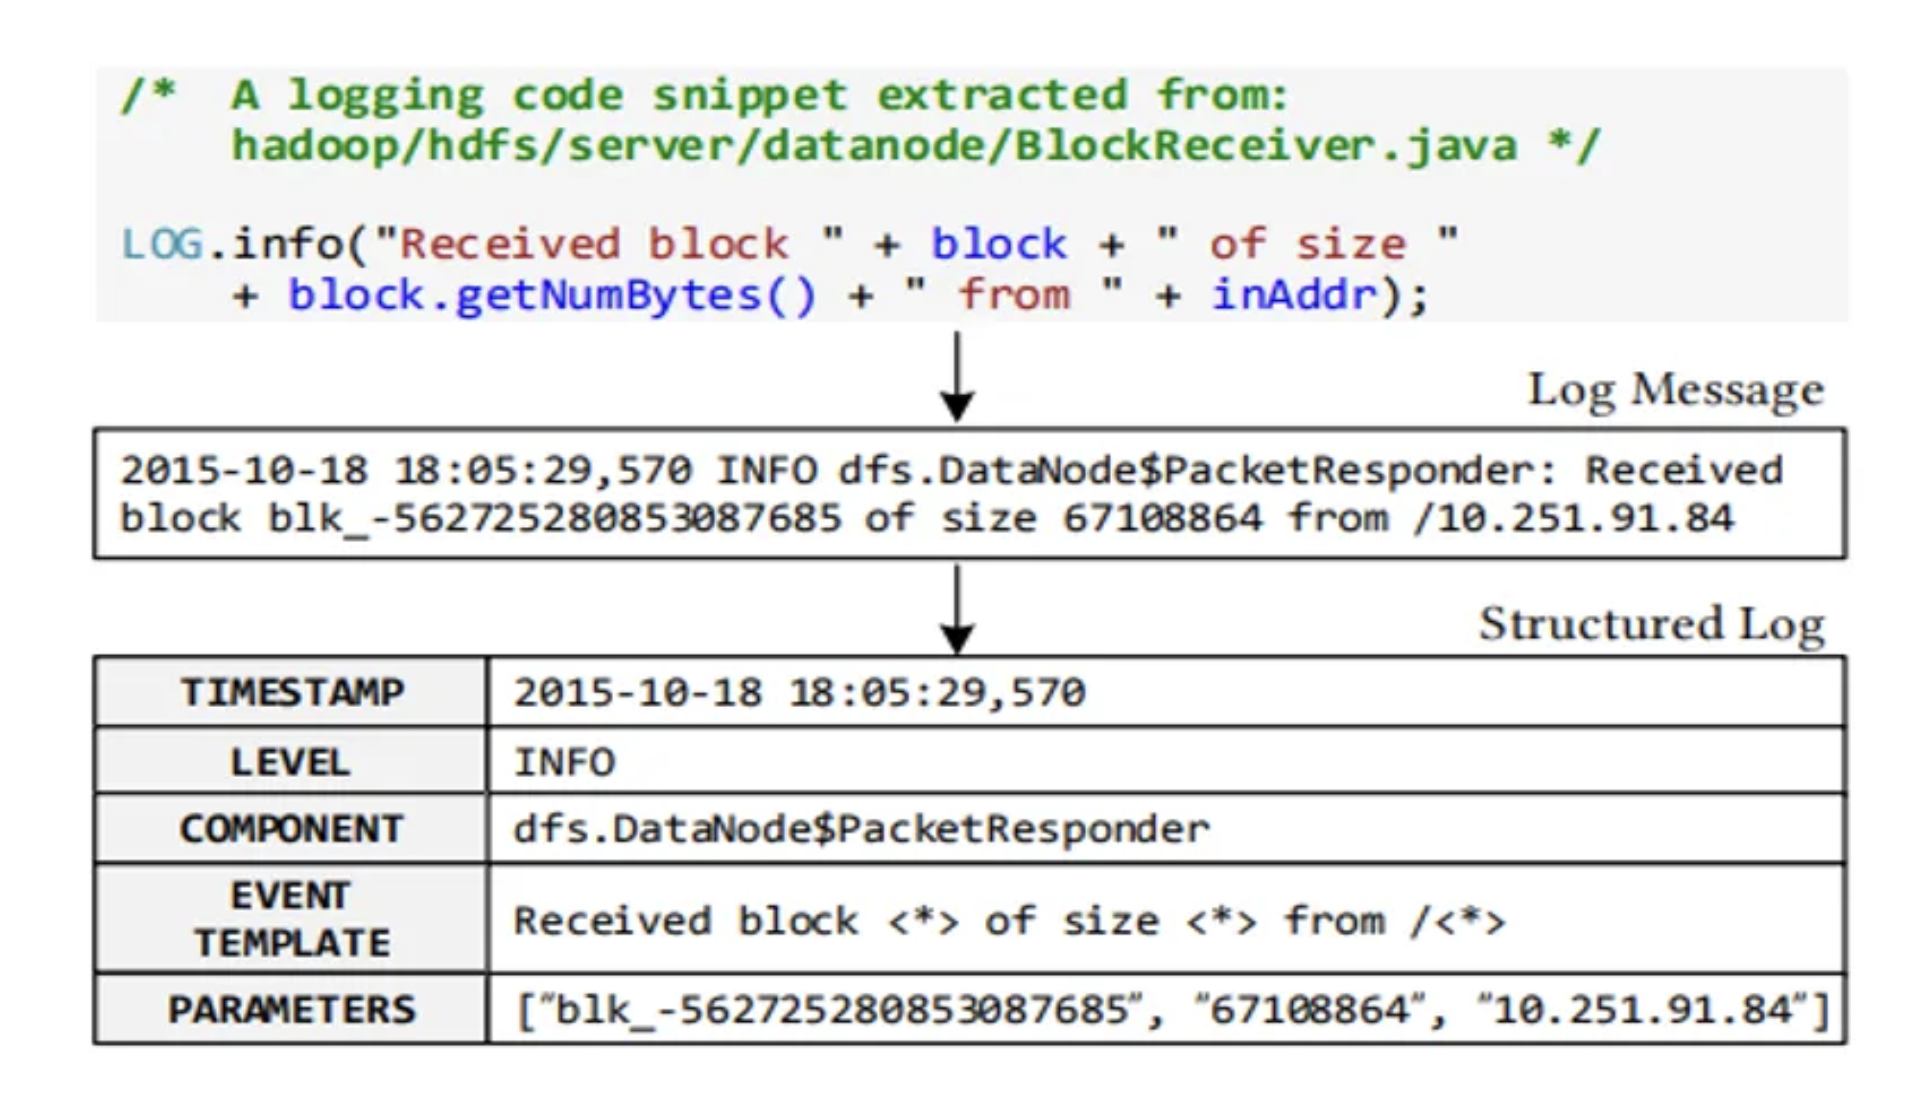
\includegraphics[width=0.95\linewidth]{drain-illustration.png}
\caption{DRAIN parsing: from raw log to structured template (variables masked, fixed skeleton preserved).}
\label{fig:drain}
\end{figure}

LogBERT~\cite{guo2021logbert} trains a Transformer on log-key sequences with MLKP (masked log-key prediction, ratio $m$) and VHM (compactness of normals). Paper-style scoring: for each masked position, an error is counted when the observed key falls outside the top-$g$ candidates; a session is anomalous when its error proportion exceeds $r$. The same $m$ is used in training and inference.

\subsection{Comparison with Existing Methods (LogBERT Paper SOTA)}

The LogBERT paper~\cite{guo2021logbert} evaluates six baselines from three families on HDFS, BGL and Thunderbird: count-vector + classical detector methods (\textbf{PCA}~\cite{xu2009detecting}, \textbf{One-Class SVM}~\cite{scholkopf2001estimating}, \textbf{Isolation Forest}~\cite{liu2008isolationforest}, \textbf{LogCluster}~\cite{lin2016logcluster}) and recurrent networks (\textbf{DeepLog}~\cite{du2017deeplog}, \textbf{LogAnomaly}~\cite{meng2019loganomaly}). All use Drain~\cite{he2017drain} for parsing; PCA/OCSVM/iForest/LogCluster are evaluated via Loglizer~\cite{he2016experience}. Table~\ref{tab:sota-hdfs} reproduces the paper's HDFS figures (Table~2, test with 553,366~normal / 10,647~anomalous sequences).

\begin{table}[H]
\centering
\begin{tabular}{lccc}
\toprule
Method & Precision & Recall & F1 \\
\midrule
PCA & 0.0589 & 1.0000 & 0.1112 \\
Isolation Forest & 0.5360 & 0.6941 & 0.6049 \\
OCSVM & 0.0254 & 1.0000 & 0.0495 \\
LogCluster & 0.9926 & 0.3708 & 0.5399 \\
DeepLog & 0.8844 & 0.6949 & 0.7734 \\
LogAnomaly & 0.9415 & 0.4047 & 0.5619 \\
\textbf{LogBERT (paper)} & \textbf{0.8702} & \textbf{0.7810} & \textbf{0.8232} \\
\bottomrule
\end{tabular}
\caption{State of the art on HDFS after Guo et al. (2021), Table~2. Source: \texttt{2103.04475v1.pdf}.}
\label{tab:sota-hdfs}
\end{table}

Reading: count-based methods sacrifice temporal order (PCA/OCSVM at recall 1.0 but near-zero precision); LogCluster rises in precision but misses half the anomalies; DeepLog and LogAnomaly confirm the value of sequential modelling, with the best classical F1 at 0.7734 (DeepLog). LogBERT (0.8232) outperforms them with superior precision/recall balance. The paper's ablation (Table~3) explains this gain: MLKP alone yields 0.7754 / 0.7865 / 0.7809, VHM alone 0.0243 / 0.3917 / 0.0458, and combined MLKP+VHM 0.8702 / 0.7810 / 0.8232 --- VHM contributes +4.2~pts of F1 on HDFS with short sequences (average length 19), where its contribution is marginal on BGL/Thunderbird with long sequences. Our V1/V2 protocol reuses this foundation identically (same top-$g$/$r$ scoring, same $m$ in training and inference) before testing its sensitivity to $m$.

\textbf{Paper baseline (Guo et al., 2021, HDFS): Precision 87.02\%, Recall 78.10\%, F1 82.32\%.} Indicative, non-paired reference: different split, official predictor threshold tuned on test, 4 layers in the code vs.\ 2 described. Repository: \url{https://github.com/HelenGuohx/LogBERT.git}, commit \texttt{a845e61}~\cite{logbert-repo}.

\section{Pipeline Architecture}

\begin{figure}[htbp]
\centering
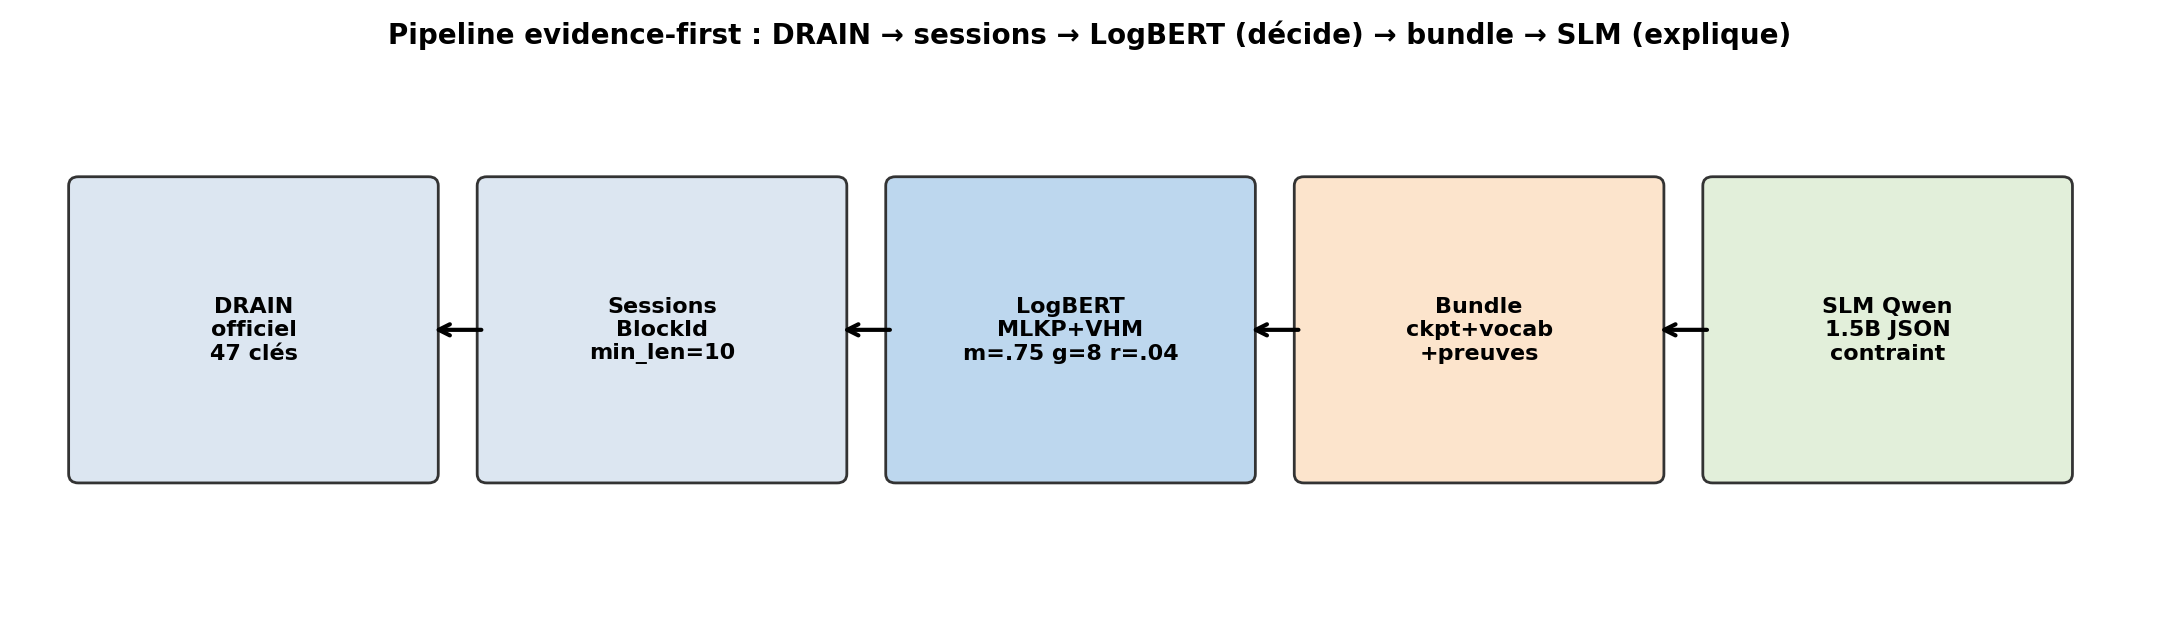
\includegraphics[width=0.95\linewidth]{fig_pipeline.png}
\caption{Evidence-first funnel architecture. LogBERT decides; the deterministic policy filters; the SLM explains.}
\label{fig:pipeline}
\end{figure}

Five stages: (1)~official DRAIN parsing $\rightarrow$ 47 keys; (2)~sessionisation by \texttt{BlockId}, \texttt{min\_len}=10; (3)~LogBERT MLKP+VHM; (4)~AIOps bundle (\texttt{best\_bert.pth}, \texttt{vocab.pkl}, Drain mapping, \texttt{inference.py}, manifest) with an API over \texttt{EventId} sequences; (5)~Qwen2.5-1.5B-Instruct SLM in constrained JSON (engineer summary, LogBERT reading, probable causal chain, uncertainties, P1--P3 actions, cited events). The SLM never re-decides; any free-form action is forbidden (finite catalogue + deterministic parameter injection), with a single reading direction: the further right in Figure~\ref{fig:pipeline}, the less data and the more qualified its content.

\section{Experimental Protocol}

Kaggle GPU T4. HDFS\_v1 data (Zenodo 8196385, MD5 \texttt{76a24b4d9a6164d543fb275f89773260}), logpai/loglizer labels. \textbf{Normal-only training}: 4,855 sessions (seed-20 shuffle from the official script). \textbf{Validation}: 55,336 normal / 2,139 anomalous. \textbf{Locked test}: 498,032 / 8,508 (1.68\% prevalence), disjoint \texttt{BlockId}s, 575,061 sessions and 11,175,629 events in total (median 19, p95 28). Vocabulary derived from training only. Selection of $m,g,r$ on validation (projection at reference prevalence); test metrics at real prevalence + 95\% Wilson intervals.

V2 grid: $m \in \{0{.}50, 0{.}65, 0{.}75\}$, $g \in \{1,\dots,15\}$, $r \in [0,0{.}80]$ step 0.01, single seed. V1 = official baseline $m{=}0{.}65,g{=}6,r{=}0$. Compatibility fixes with no model change: \texttt{torch.\_six}, \texttt{np.float/int/Inf}, ragged \texttt{dtype=object}, pandas 2.2.3 / NumPy 2.x.

\section{Training: Train / Validation Curves}

\begin{figure}[htbp]
\centering
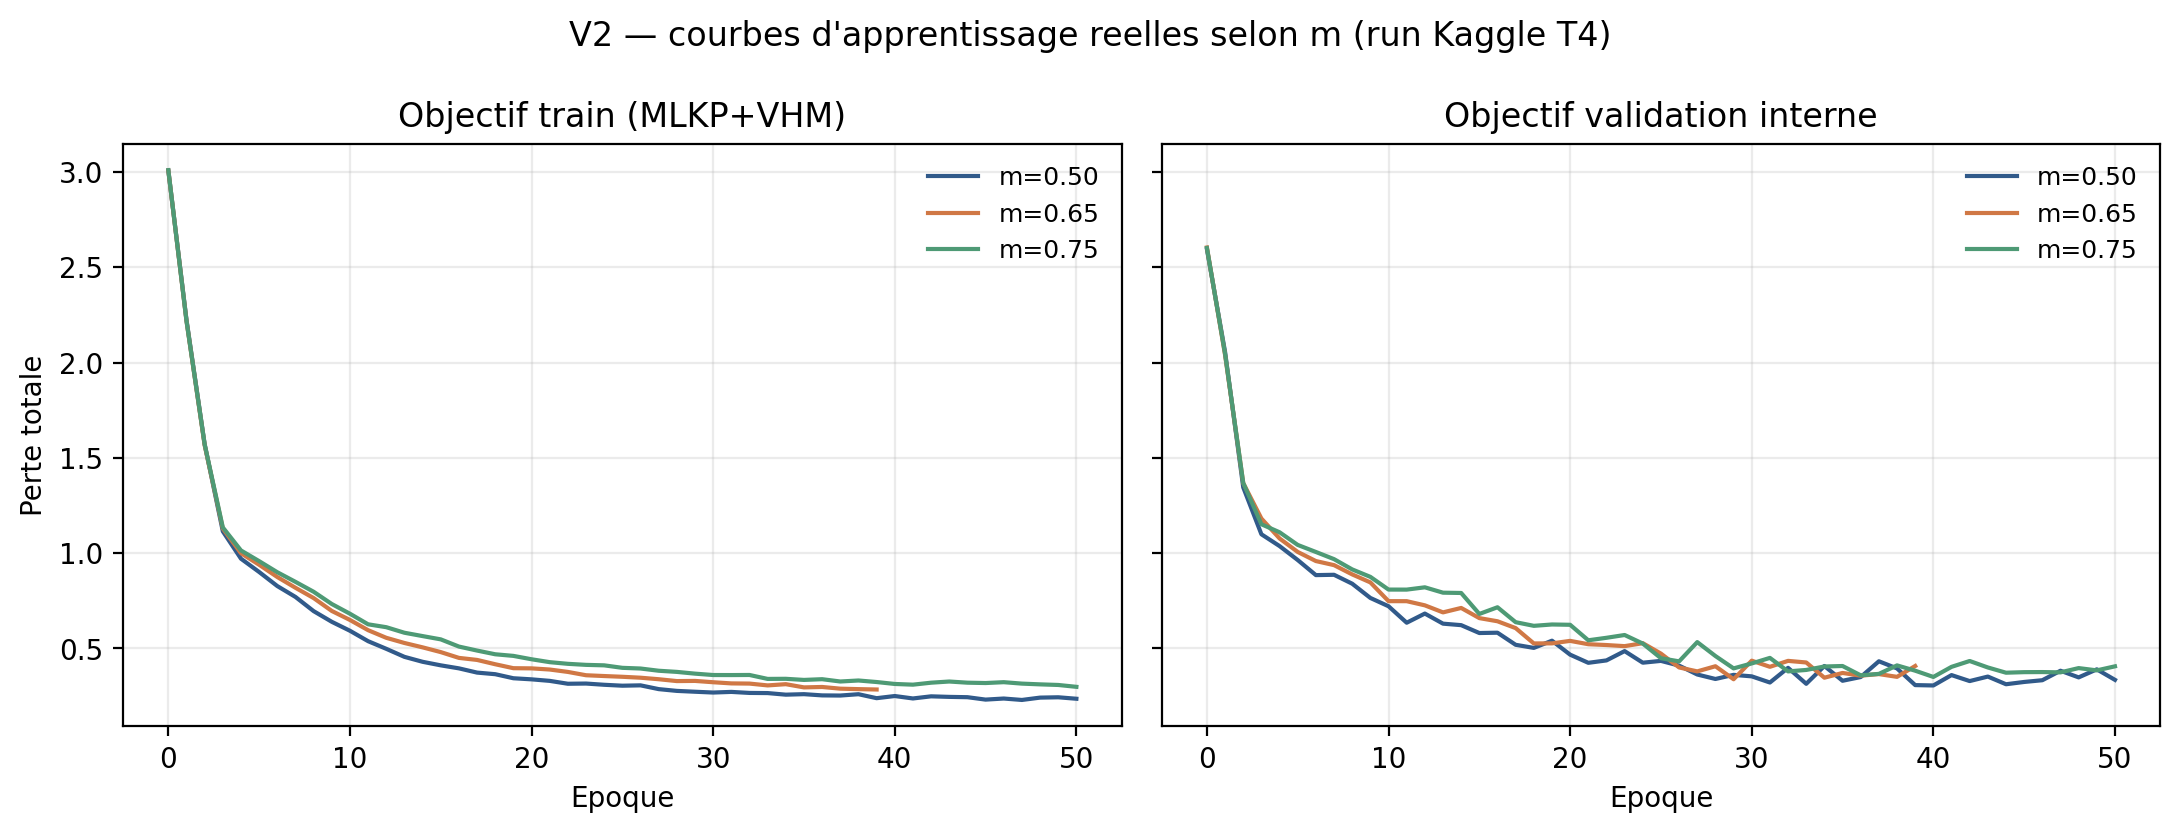
\includegraphics[width=0.95\linewidth]{fig_loss_train_val.png}
\caption{Real total MLKP+VHM objective curves (Kaggle run). Train: 0.2356 ($m{=}0{.}50$), 0.2842 ($m{=}0{.}65$, early stop at 40 epochs), 0.2982 ($m{=}0{.}75$); internal validation: 0.3348 / 0.4075 / 0.4058. Minimum loss ($m{=}0{.}50$) does not give the best detection.}
\label{fig:loss}
\end{figure}

The initial drop is shared by all three curves and the train/validation gap stays stable; the triplet $m{=}0{.}75,g{=}8,r{=}0{.}04$ maximises validation F1 (0.8493), with test F1 at 0.8314 ($-$1.8~pts, healthy generalisation).

Engineer's reading: fast convergence (drop from $\sim$3.0 to $<$1.0 in $\sim$5 epochs), then plateau; stable train/validation gap ($\sim$0.10) with no explosive divergence thanks to NLL capping; effective early stopping for $m{=}0{.}65$. Most importantly, \textbf{the best MLKP is not the best detector}: selection uses validation F1, not loss (Figure~\ref{fig:selection}).

\begin{figure}[htbp]
\centering
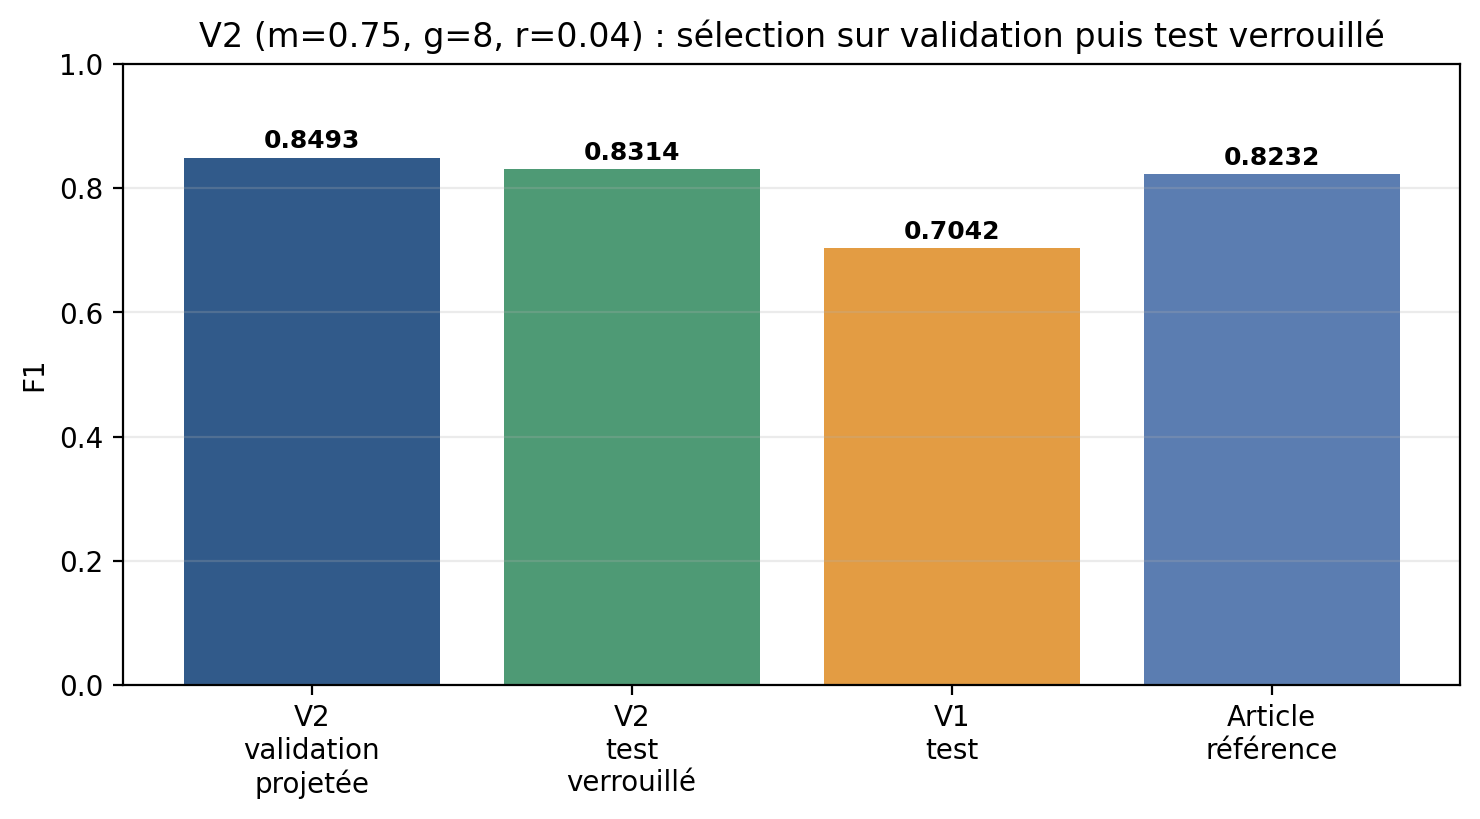
\includegraphics[width=0.85\linewidth]{fig_selection_m.png}
\caption{Validation-only selection then locked test: projected validation F1 of 0.8493 for triplet $m{=}0{.}75,g{=}8,r{=}0{.}04$ (projected precision 0.8677, recall 0.8317), test F1 0.8314. Test is scored only after freezing.}
\label{fig:selection}
\end{figure}

\section{Locked-Test Results}

Figures~\ref{fig:comparaison} and~\ref{fig:confusion} frame Table~\ref{tab:comparaison}.

\begin{figure}[htbp]
\centering
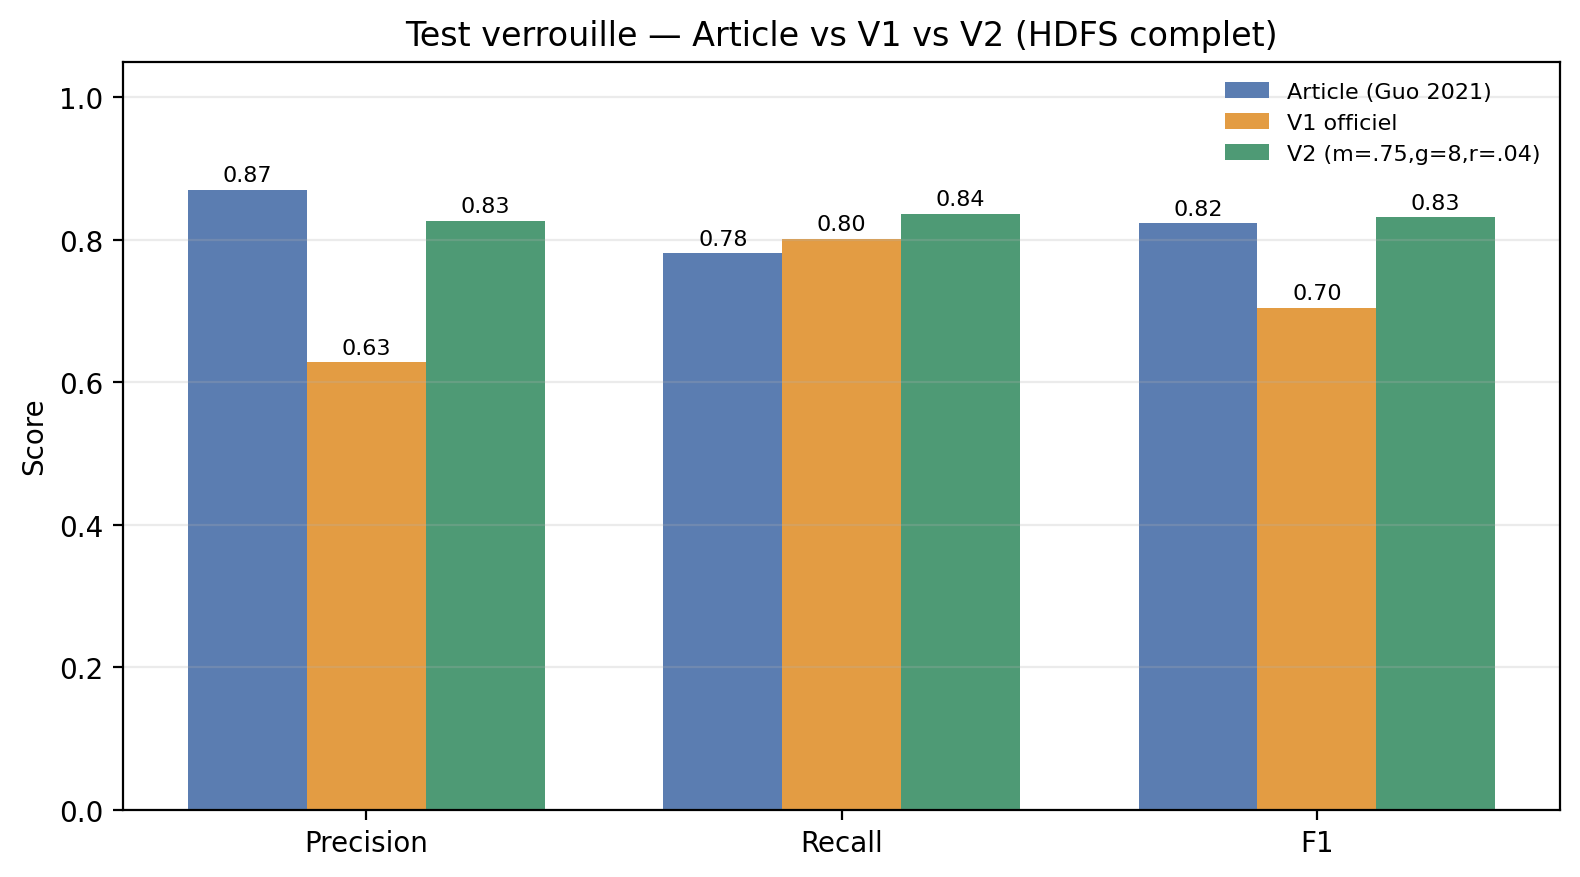
\includegraphics[width=0.95\linewidth]{fig_comparaison.png}
\caption{Locked full-HDFS test: paper (non-paired reference) vs.\ official V1 vs.\ V2.}
\label{fig:comparaison}
\end{figure}

\begin{table}[h]
\centering
\caption{Locked-test comparison. Paper: indicative reference.}
\label{tab:comparaison}
\renewcommand{\arraystretch}{1.35}
\begin{tabular}{lccccc}
\toprule
Version & Precision & Recall & F1 & ROC-AUC & PR-AUC \\
\midrule
Paper HDFS & 0.8702 & 0.7810 & 0.8232 & --- & --- \\
V1 ($m{=}0{.}65,g{=}6,r{=}0$) & 0.6278 & 0.8017 & 0.7042 & 0.8979 & 0.6338 \\
\textbf{V2 ($m{=}0{.}75,g{=}8,r{=}0{.}04$)} & \textbf{0.8267} & \textbf{0.8362} & \textbf{0.8314} & \textbf{0.9235} & \textbf{0.7051} \\
\bottomrule
\end{tabular}
\end{table}

\begin{figure}[htbp]
\centering
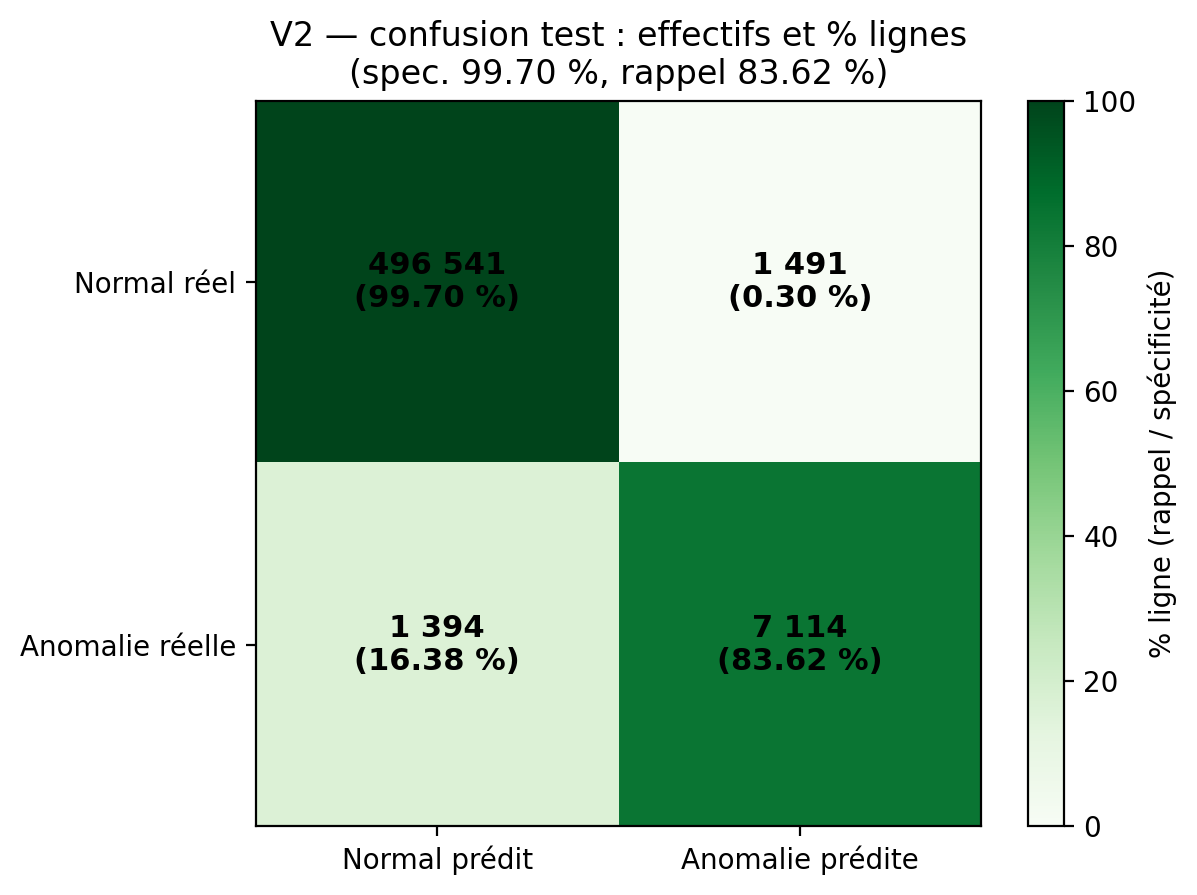
\includegraphics[width=0.75\linewidth]{fig_confusion.png}
\caption{V2 matrix in counts and row \%: 496,541 correctly classified normals (99.70\%) and 7,114 detected anomalies (83.62\%); 1,491 FPs (0.30\%) and 1,394 FNs (16.38\%).}
\label{fig:confusion}
\end{figure}

V2 detail: Precision 95\% CI [0.8186; 0.8346], Recall 95\% CI [0.8281; 0.8439], FPR 0.0030, Accuracy 0.9943, \textbf{Balanced accuracy 0.9166}, Specificity 0.9970. Validation $\rightarrow$ test gap: 0.8493 $\rightarrow$ 0.8314 ($-$1.8~pts), healthy generalisation.

\textbf{Reading:} V2 beats V1 by +19.9~pts (P), +3.4~pts (R), +12.7~pts (F1), FPR $\div$2.7. Against the paper: R +5.5~pts, F1 +0.8~pt, P $-$4.35~pts = \textbf{partial exceedance only}. Single seed: insufficient to claim robust superiority (requires 3--5 seeds, mean $\pm$ std).

\section{BGL Generalisation and Multi-Seed Rigor (V3)}

Same protocol as V2 (official repository \texttt{a845e61}, paper-style scoring, normal-only training, validation selection, locked test), applied to \textbf{BGL}: 4.7~million BlueGene/L messages, 5-min sliding windows / 1-min step (average length $\sim$562 vs.\ $\sim$19 for HDFS), seed-12 shuffle, \texttt{train\_ratio=0.4}. Split: 6,681 normal training sessions; validation 1,010 / 535; test 9,053 / 2,091 (18.76\% prevalence). Training-only vocabulary: 185~keys. Grid $m \in \{0{.}35, 0{.}50, 0{.}65\}$ around the official default $0{.}50$; seeds 1234/2026/999 on frozen splits (only initialisation, training and masking vary).

\begin{figure}[htbp]
\centering
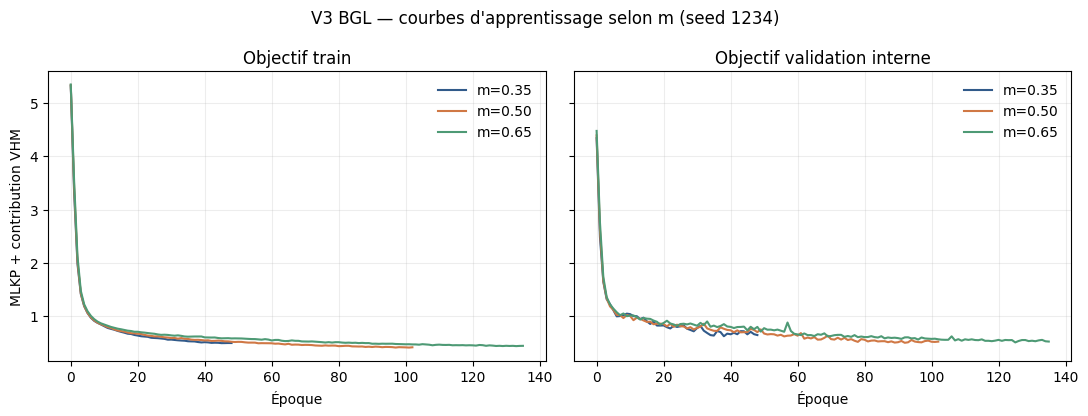
\includegraphics[width=0.95\linewidth]{fig_bgl_loss.png}
\caption{V3 BGL — MLKP+VHM curves by $m$: 49 epochs ($m{=}0{.}35$), 103 ($m{=}0{.}50$), 136 ($m{=}0{.}65$). Effective early stopping, no divergence.}
\label{fig:bgl-loss}
\end{figure}

Phase-A selection (seed~1234): \textbf{$m{=}0{.}50,g{=}15,r{=}0{.}01$} (projected validation F1 0.9119, validation $\rightarrow$ test gap $-0{.}2$~pts). Locked test per seed (Table~\ref{tab:bgl-seeds}, Figure~\ref{fig:bgl-diag}).

\begin{table}[H]
\centering
\caption{V3 BGL, locked test per seed; validation-frozen thresholds.}
\label{tab:bgl-seeds}
\renewcommand{\arraystretch}{1.35}
\begin{tabular}{lcccccc}
\toprule
Seed & Precision & Recall & F1 & FPR & ROC-AUC & PR-AUC \\
\midrule
1234 & 0.9046 & 0.9158 & 0.9102 & 0.0223 & 0.9595 & 0.9189 \\
2026 & 0.8979 & 0.9168 & 0.9072 & 0.0241 & 0.9595 & 0.9187 \\
999 & 0.9112 & 0.9173 & 0.9142 & 0.0207 & 0.9597 & 0.9183 \\
\midrule
Mean ± std (n=3) & 0.9045±0.0066 & 0.9166±0.0007 & 0.9105±0.0035 & 0.0223±0.0017 & 0.9596±0.0001 & 0.9187±0.0003 \\
Paper BGL & 0.8940 & 0.9232 & 0.9083 & --- & --- & --- \\
\bottomrule
\end{tabular}
\end{table}

\begin{figure}[htbp]
\centering
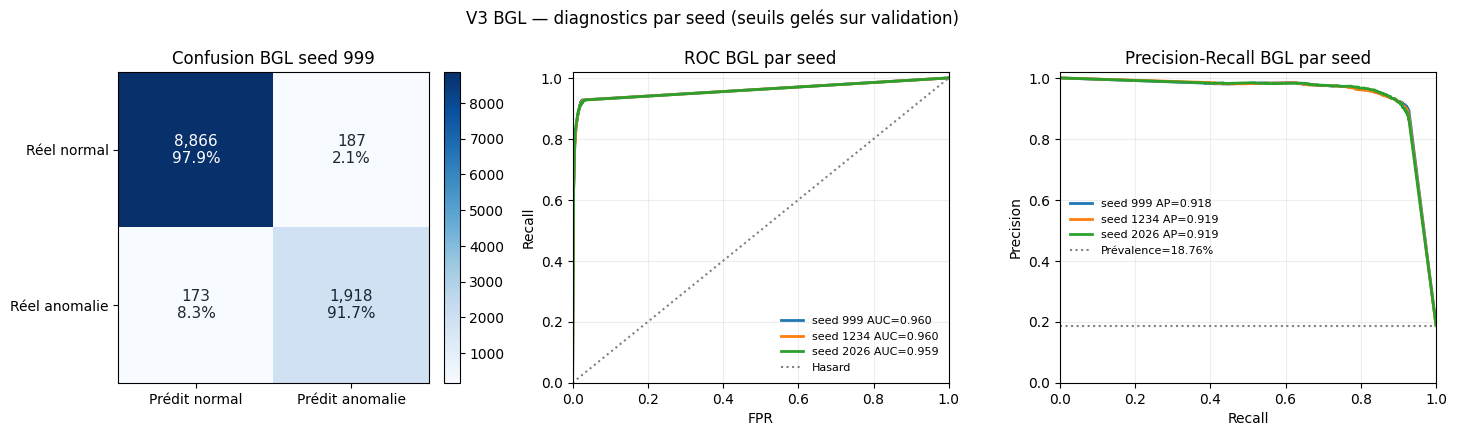
\includegraphics[width=0.95\linewidth]{fig_bgl_diag.png}
\caption{V3 BGL — best-seed (999) confusion, per-seed ROC and Precision-Recall (frozen thresholds).}
\label{fig:bgl-diag}
\end{figure}

\textbf{Reading:} against the BGL paper (89.40 / 92.32 / 90.83): P $+$1.05~pts, R $-$0.66~pts, F1 $+$0.22~pts, i.e.\ less than the inter-seed std ($\pm$0.35): \textbf{a match, not an exceedance}. Multi-seed forbids an abusive claim here — exactly its purpose. Remarkable stability (recall $\pm$0.0007, ROC $\pm$0.0001).

\begin{figure}[htbp]
\centering
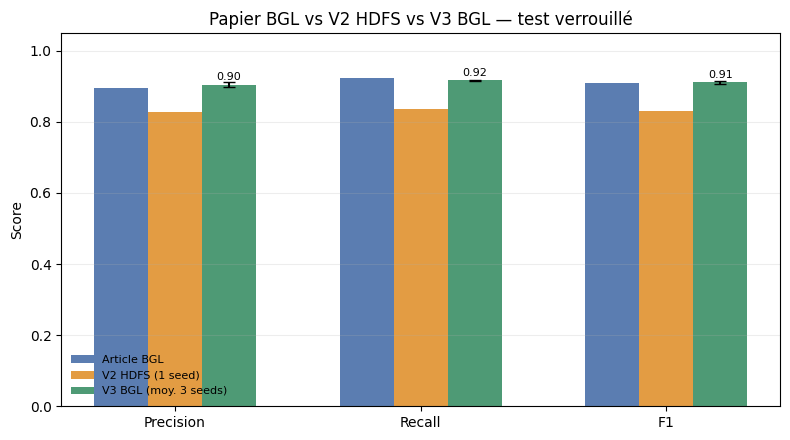
\includegraphics[width=0.95\linewidth]{fig_bgl_cross.png}
\caption{Paper BGL vs.\ V2 HDFS (1~seed) vs.\ V3 BGL (3-seed mean). Precisions are not comparable across datasets (prevalences 18.76\% vs.\ 1.68\%).}
\label{fig:bgl-cross}
\end{figure}

\textbf{Main lesson:} the optimal $m$ follows sequence length — HDFS ($\sim$19~tokens) wanted $m{=}0{.}75$, BGL ($\sim$562~tokens) confirms the official $m{=}0{.}50$ default (already masking $\sim$280~positions per session). The V2/V3 ablation thus forms a unified result rather than two ad-hoc settings. Remaining symmetry: Phase~C (extra HDFS seeds on $m{=}0{.}75$) for equal rigor on the HDFS side.

\section{Inference and Enterprise Applicability}

\subsection{Bundle Inference Contract}

Input: list of numeric \texttt{EventId}s (Drain output), \texttt{session\_id}, seed. Output: \texttt{anomaly} (score $> r$), \texttt{anomaly\_score} = out-of-top-$g$ error proportion, \texttt{masked\_tokens}, \texttt{undetected\_tokens}, \texttt{evidence} (position, \texttt{observed\_event\_id}, template, top-$g$ candidates + templates). Real smoke test: normal (15 masked, 0 errors, score 0.0 $\rightarrow$ normal); anomalous (18 masked, 1 error, 0.0556 $> 0{.}04 \rightarrow$ anomaly), evidence \texttt{Event~15} (\textit{Unexpected error trying to delete block\dots, BlockInfo not found in volumeMap}) outside the 8 expected. Latency: batched DataLoader scoring, no vocabulary recomputation; the SLM is called only on novel signatures.

\subsection{Worldline (TFI) Integration}

Target chain: collectors (Fluent Bit / Logstash) $\rightarrow$ streaming Drain normalisation $\rightarrow$ sessionisation (application window: \texttt{BlockId} here, \texttt{trace\_id} / time window in banking production) $\rightarrow$ LogBERT per application profile (one model per behaviour: payments, CRM, IAM) $\rightarrow$ SHA256 signature + deduplication + 24-h cache $\rightarrow$ alert queue (ServiceNow / PagerDuty) with evidence dossier $\rightarrow$ local SLM in JSON $\rightarrow$ mandatory human validation (human-in-the-loop). MLOps: model registry, drift monitoring ([UNK] rate, sliding FPR), retraining on validated incidents, GitOps CI/CD.

CommerzBank retrospective: 4,600 lines over 3 components, nested causes. The pipeline brings: simultaneous rupture isolation, immediate infra-vs-application qualification (Worldline responsibility limited to the platform layer), investigation cut from 20--30~min to $<$5~min of processing ($-$75 to $-$83\% estimated, to confirm in a blind trial). Under Copartis load (172~M lines/month), measured filtering ($\sim$98.3\% discarded, 1.70\% kept) + Heaps + cache brings the SLM load down to $\sim$869 calls/day (working hypothesis).

\subsection{Enterprise Use Case and Causal-Diagnostic Example (JSON)}

Scenario: on the banking scope supervised by Client Delivery~2, an HDFS session is classified \textbf{anomalous} by LogBERT V2 ($m{=}0{.}75,g{=}8,r{=}0{.}04$, score 0.0556 $> 0{.}04$). The evidence dossier (real excerpt from the bundle smoke test) is forwarded as-is to on-call, then the SLM translates it into an actionable diagnosis without re-deciding.

{\small\begin{verbatim}
{
  "session_id": "smoke-anomaly",
  "scored": true, "anomaly": true,
  "anomaly_score": 0.0556,
  "m": 0.75, "g": 8, "r": 0.04,
  "masked_tokens": 18, "undetected_tokens": 1,
  "evidence": [{
    "position": 19,
    "observed_event_id": "15",
    "observed_template": "Unexpected error trying to delete
      block blk_<*>. BlockInfo not found in volumeMap.",
    "top_g_candidate_ids": ["5","2","4","10","6","9","3","8"]
  }]
}
\end{verbatim}\par}

The Qwen2.5-1.5B-Instruct SLM answers \textbf{only} in the constrained schema below (format enforced by the prompt; illustrative content, consistent with the evidence above):

{\small\begin{verbatim}
{
  "engineer_summary": "Block deletion failure: the
    DataNode cannot find the block in its local table.",
  "logbert_reading": "Event 15 outside the expected top-8
    (block deletion/addition/verification).",
  "probable_causal_chain": "Deletion order -> block
    missing from volumeMap -> unexpected error.",
  "uncertainties": ["Block already deleted?",
    "NameNode/DataNode desync?", "Corrupted disk?"],
  "recommended_actions": [
    {"action": "VERIFY_BLOCK_REPLICATION",
     "why": "confirm block presence",
     "priority": "P1"},
    {"action": "CHECK_DATANODE_VOLUME_MAP",
     "why": "check local consistency",
     "priority": "P2"}
  ],
  "cited_events": ["15"],
  "logbert_score": 0.0556,
  "threshold_r": 0.04,
  "margin_over_threshold": 0.0156
}
\end{verbatim}\par}

Verified guardrails: cited events $\in$ LogBERT dossier, fact/hypothesis separation, actions from the finite catalogue, mandatory human validation before any execution.

Deliberate choice: no generative confidence score is requested from the SLM --- a self-assessed value from a language model is neither calibrated nor actionable for on-call. The only decision-strength signal is LogBERT's: \texttt{anomaly\_score} against threshold $r$ (here $0{.}0556 > 0{.}04$, margin $+0{.}0156$) plus the number of out-of-top-$g$ positions. Uncertainty is stated in plain text under \texttt{uncertainties}, not as a pseudo-probability. In production, this dossier flows through ServiceNow/PagerDuty with score, top-$g$ evidence and Drain templates attached.

\subsection{FinOps and Sovereignty}

\begin{figure}[htbp]
\centering
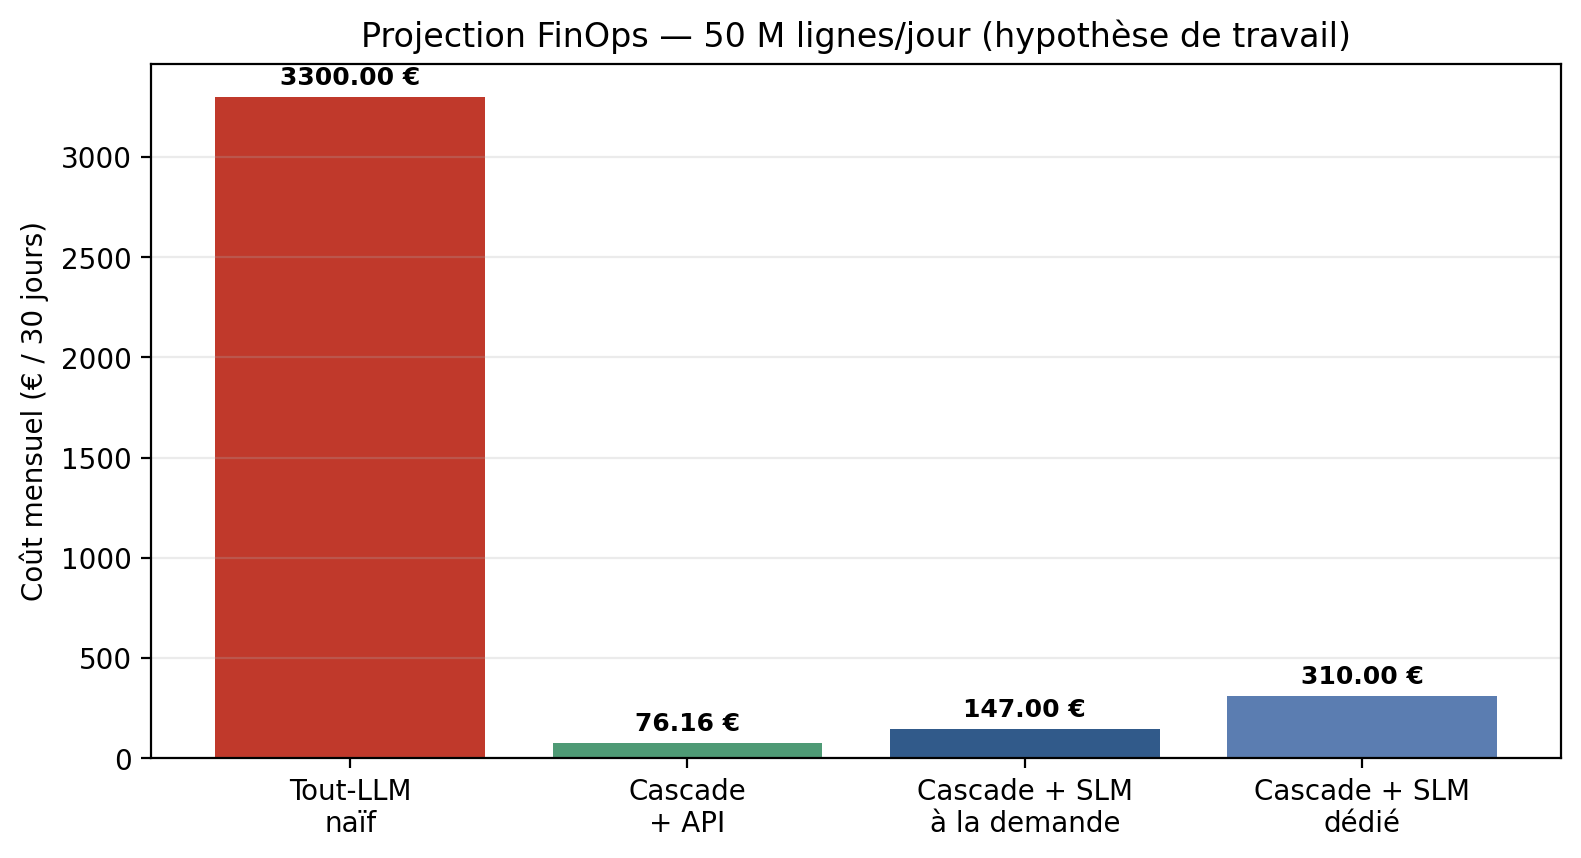
\includegraphics[width=0.9\linewidth]{fig_finops.png}
\caption{Monthly projection at 50~M lines/day: \texteuro 3,300 (naive all-LLM) vs.\ \texteuro 76.16 (cascade+API) vs.\ \texteuro 147 (cascade+self-hosted SLM on demand) vs.\ \texteuro 310 (dedicated).}
\label{fig:finops}
\end{figure}

Naive/hybrid ratio $\approx \times 43$. Sovereignty surcharge $\approx$ +\texteuro 71/month ($\times 1{.}9$): the price of data never leaving the premises (GDPR, PCI-DSS). Dedicated-vs-API break-even $\sim$785~M lines/day. The local SLM (Qwen2.5-1.5B, $\sim$34.4~s/diagnosis, 8.3~GPU-h/day, 35\% occupancy) is a compliance choice, not a marginal cost optimisation.

\subsection{Risks, Limitations, Acceptability}

Hallucinations neutralised by strict JSON + finite catalogue + deterministic injection; syntactic drift tracked via [UNK]. Limitations: single seed, non-paired paper comparison, NameNode-vs-DataNode attribution bias (fix by injecting cluster topology into context), HDFS-only evaluation to extend to multi-service. Acceptability: evidence dossier attached to every alert, supervised advisor mode.

\section{Conclusion}

Locked V2: \textbf{0.8267 / 0.8362 / 0.8314} (1~seed), ROC-AUC 0.9235, PR-AUC 0.7051, FPR 0.30\% over 506,540 sessions; V3 BGL: \textbf{0.9045 / 0.9166 / 0.9105} (3-seed mean, $\pm$0.0035 in F1), matching the BGL paper (90.83). Hybridisation reconciles detection, constrained explainability and sustainability ($\div 43$, \texteuro 76--147/month). Partial paper exceedance, to consolidate with multi-seed repeats. Recommendations: per-profile MLOps registry, FinOps-by-design ($<$1,000 calls/day), human-in-the-loop, blind MTTR measurement.

\begin{thebibliography}{99}
\bibitem{vaswani2017attention} Vaswani et al. Attention is all you need. NeurIPS, 2017.
\bibitem{kingma2013vae} Kingma, Welling. Auto-encoding variational Bayes. ICLR, 2013.
\bibitem{devlin2018bert} Devlin et al. BERT. NAACL, 2018.
\bibitem{he2017drain} He et al. Drain: online log parsing with fixed depth tree. ICWS, 2017.
\bibitem{guo2021logbert} Guo et al. LogBERT: log anomaly detection via BERT. IJCNN, 2021.
\bibitem{logbert-repo} Official LogBERT repository. \url{https://github.com/HelenGuohx/LogBERT.git}, commit \texttt{a845e61}.
\bibitem{zhu2019tools} Zhu et al. Tools and benchmarks for automated log parsing. ICSE-SEIP, 2019.
\bibitem{he2020loghub} He et al. Loghub: a large collection of system log datasets. ISSRE, 2020.
\bibitem{du2017deeplog} Du et al. DeepLog: anomaly detection and diagnosis from logs. CCS, 2017.
\bibitem{xu2009detecting} Xu et al. Online system problem detection by mining patterns of console logs. ICDM, 2009.
\bibitem{scholkopf2001estimating} Sch\"olkopf et al. Estimating the support of a high-dimensional distribution. Neural Computation, 2001.
\bibitem{liu2008isolationforest} Liu et al. Isolation Forest. ICDM, 2008.
\bibitem{lin2016logcluster} Lin et al. Log clustering based problem identification for online service systems. ICSE, 2016.
\bibitem{he2016experience} He et al. Experience report: system log analysis for anomaly detection. ISSRE, 2016.
\bibitem{meng2019loganomaly} Meng et al. LogAnomaly: unsupervised detection of sequential and quantitative anomalies. IJCAI, 2019.
\bibitem{xu2010mining} Xu et al. Detecting large-scale system problems by mining console logs. SOSP, 2009.
\bibitem{ndichu2026} Ndichu et al. Alert fatigue in production supervision, 2026.
\bibitem{ji2023hallucination} Ji et al. Survey of hallucination in NLG. ACM Comp. Surv., 2023.
\bibitem{qwen2025} Qwen Team. Qwen2.5 technical report, 2025.
\bibitem{llama3} Meta AI. Llama 3 model card, 2024.
\bibitem{heaps1978} Heaps. Information retrieval. Academic Press, 1978.
\bibitem{han2022ervised} Han et al. A survey on AIOps for failure management. ACM Comp. Surv., 2022.
\bibitem{notaro2021aion} Notaro et al. AIOps: chronology, landscape and challenges. IEEE Trans. Net. Serv. Manag., 2021.
\bibitem{worldline-deu2024} Worldline. Universal registration document 2024. Worldline Investors, revenue \texteuro 4,632~M, $\sim$18,000 experts, $\sim$40 countries. \url{https://investors.worldline.com/}.
\bibitem{worldline-site} Worldline. PayTech provider, services to financial institutions and locations. \url{https://worldline.com/}.
\end{thebibliography}

\end{document}
